\documentclass[a4paper,12pt,notitlepage]{article}
\usepackage{mathtools}
\usepackage{amssymb}
\usepackage{braket}
\usepackage{graphicx}
\usepackage[section]{placeins}
\title{Data Analysis}
\author{Richard Fox}
\date{}

\begin{document}

\maketitle

\section{Analysing Exoplanet Data}

Starting off with the naive approach, just finding the local minima and averaging the distance between them (Figure 1), yielding an orbital period of 2.2 days, presuming the measurements are recorded in days. 

\begin{figure}[h]
    \centering
    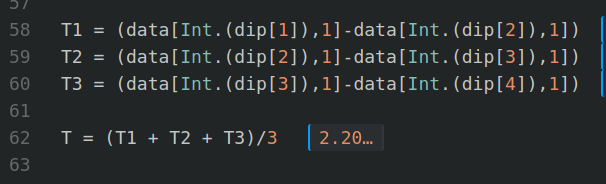
\includegraphics[width=\textwidth]{Period.png}
    \caption{dip is an array holding all of the argmin() functions relating to the large intensity dips}
    \label{fig:my_label}
\end{figure}

Next an attempt to show this using an fft algorithm is attempted, but it seems to correspond to a period of $\approx 4.822$ days which cannot be correct, although there is a much smaller peak corresponding to  the 2.2 period.

\begin{figure}[h]
    \centering
    \begin{minipage}{0.5\textwidth}
        \centering
        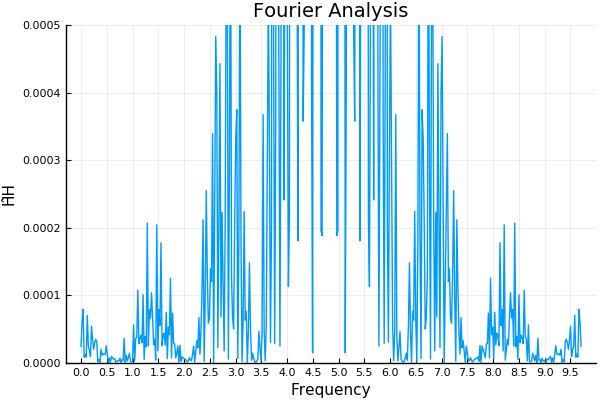
\includegraphics[width=0.9\textwidth]{ftfull.png} 
    \end{minipage}\hfill
    \begin{minipage}{0.5\textwidth}
        \centering
        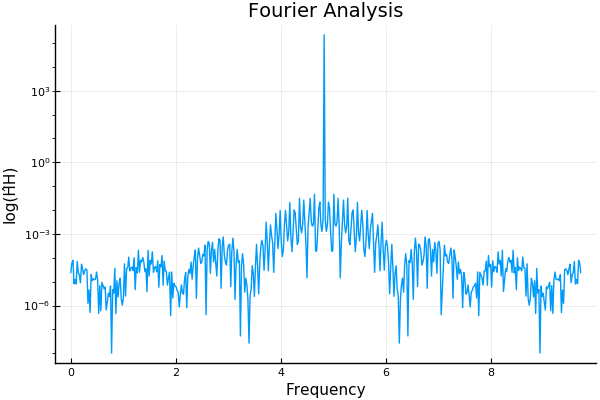
\includegraphics[width=0.9\textwidth]{logfull.png} 
    \end{minipage}
\end{figure}

Furthermore, there is a vast peak,that I believe corresponds to the frequency for the orbital period, even if the much smaller spikes seem to match half wavelength harmonics of a 2.2 day period.

\begin{figure}[h]
    \centering
    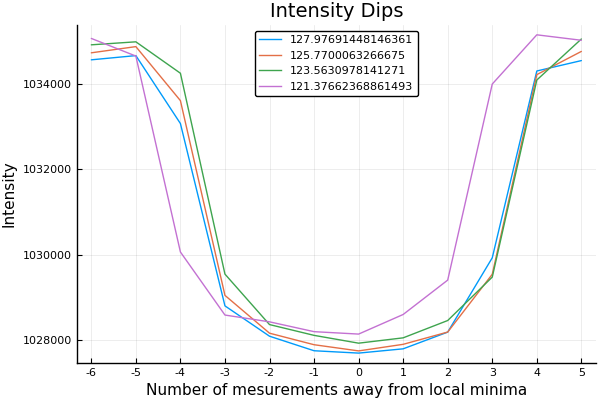
\includegraphics[width=\textwidth]{dips.png}
    \caption{curves are denoted by the measurement number at which the minima is found}
\end{figure}

By plotting the intensity dips (Figure 2) over the same range we can extrapolate the points at which the exoplanet starts blocking light and when it ends. By take the average of the points we get a transit time of $\approx 0.1839$ days or $\approx 4.41$ hours (Figure 3).

\begin{figure}[h]
    \centering
    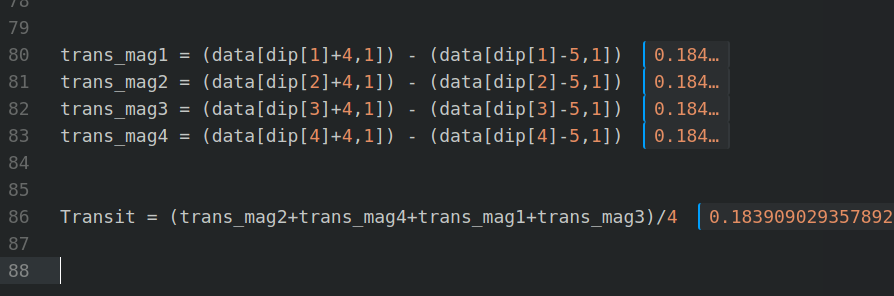
\includegraphics[width=\textwidth]{Transit.png}
    \caption{Calculated by taking the average of the duration of the times when intensity is significantly lower than average Intensity}
\end{figure}

Flux is given by $flux = \frac{Intensity}{Area}$ as we don't know the areas we can only find the ratio of the star and planet radii. 
$$ \frac{I_s}{A_s} = \frac{I_{s-p}}{A_s-A_p} $$
where $I_s\   ,  I_{s-p}$ are the intensity of the sun and of the sun when the planet passes respectively, $A_s\  ,  A_p$ are the area of the sun and planet respectively. The astronomical distance away any star is we can treat the area as a circle giving the ratio of radii as:
$$\frac{r_s}{r_p} = \sqrt{1-\frac{I_{s-p}}{I_s}}$$

\begin{figure}[h]
    \centering
    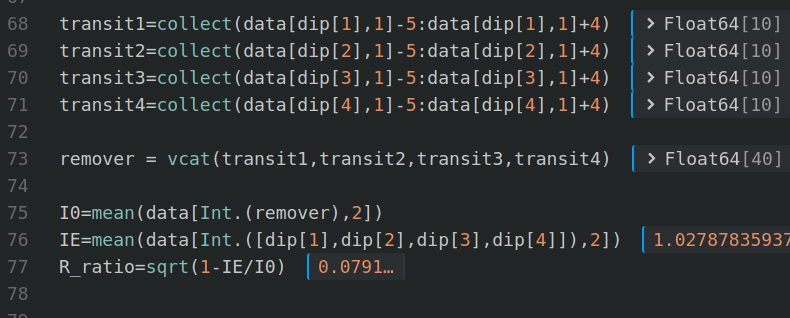
\includegraphics[width=\textwidth]{radii.png}
    \caption{remover is present to remove the data when the planet is in front of the star allowing for a meaningful average of intensity without an obstructing body}
\end{figure}

Which is shown by R\_ratio in (Figure 4), corresponding to the star being only $11.75$ times larger than its planet! Considering the Sun is $400$ times larger than the earth, and the Sun is $10$ times larger by radius than Jupiter, I would like to start to try and make simple hypotheses on this system.

By considering the period of 2.2 days, we can infer a relative velocity, and can constrict this by a relative escape velocity, or restrict the mass of the planet but using Jupiter as the largest dimension of planet for condensing and beginning to become a star occurs. However upon thinking about this our data actually does not give us any information on parallax between these bodies. There, to my knowledge, is no difference between the observed intensities if the star is orbiting the planet or vice versa and therefore it could have more or less mass than Jupiter, as Jupiter would shrink as it acquired more mass from its current size. Meaning, disappointingly, I can make no further meaningful deductions.

However from some online research I have found this article\\ [http://sac.au.dk/fileadmin/www.sac.au.dk/Project\_updated\_gr.1.pdf]\\
which leads me to believe I have data from the exoplanet HAT-P-7, however the power spectrum I produced is rather closer to the exoplanet Kepler-7b. Curious. Further investigation needed. Although it does confirm my hypothesis of the planet being Jupiter-like, referring to it specifically as a 'Hot Jupiter' which is a Jupiter-like planet with an orbit of $< 10$ days.


\section{Simulation of an Auto-Regressive Model}

\begin{figure}[h]
    \centering
    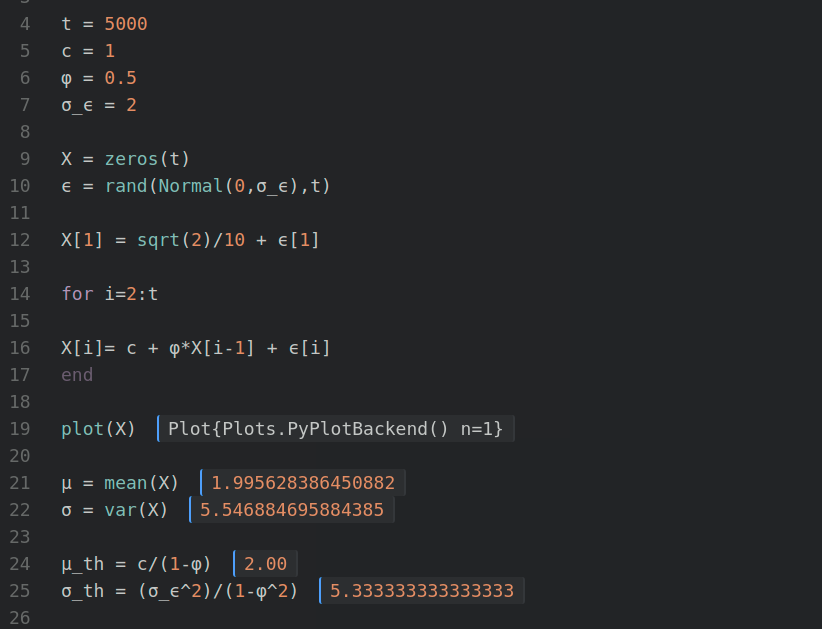
\includegraphics[width=\textwidth]{th_em.png}
    \caption{The value of this sample are close to but not quite equal to the theoretical values as we would expect from a sample of a distribution}
\end{figure}

\begin{figure}[h]
    \centering

        \centering
        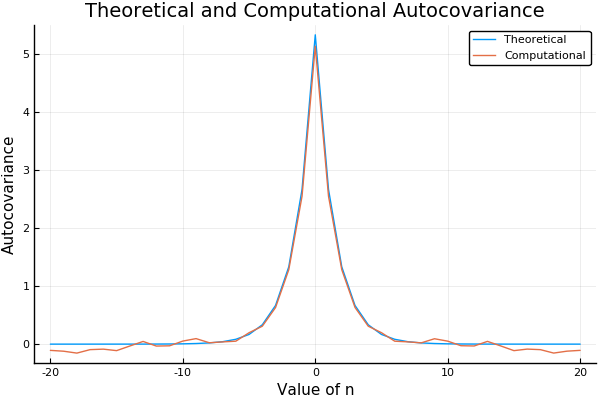
\includegraphics[width=0.9\textwidth]{smallautocov.png}
        \caption{Matches quite well but is seeming to deviate as n grows}
\end{figure}

\begin{figure}
        \centering
        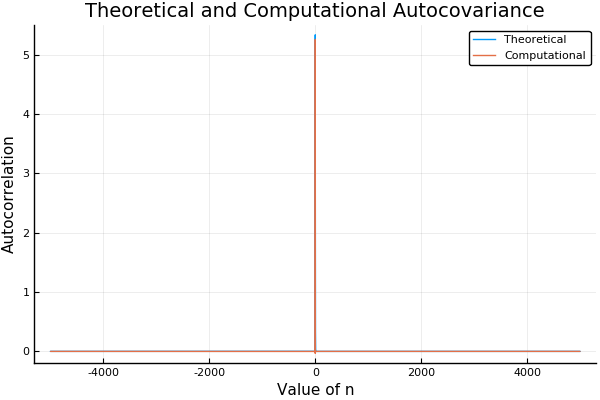
\includegraphics[width=0.9\textwidth]{largeautocov.png}
        \caption{Deviates wildly as we get to larger n, but as we have less data points this is to be expected. At the outer most edges it is almost a standard deviation away from the expected 0, in some cases, but again this makes sense as sample size is tending to 1}

\end{figure}




\end{document}